\documentclass[9pt,letterpaper]{article}\usepackage[]{graphicx}\usepackage[]{color}
% maxwidth is the original width if it is less than linewidth
% otherwise use linewidth (to make sure the graphics do not exceed the margin)
\makeatletter
\def\maxwidth{ %
  \ifdim\Gin@nat@width>\linewidth
    \linewidth
  \else
    \Gin@nat@width
  \fi
}
\makeatother

\definecolor{fgcolor}{rgb}{0.345, 0.345, 0.345}
\newcommand{\hlnum}[1]{\textcolor[rgb]{0.686,0.059,0.569}{#1}}%
\newcommand{\hlstr}[1]{\textcolor[rgb]{0.192,0.494,0.8}{#1}}%
\newcommand{\hlcom}[1]{\textcolor[rgb]{0.678,0.584,0.686}{\textit{#1}}}%
\newcommand{\hlopt}[1]{\textcolor[rgb]{0,0,0}{#1}}%
\newcommand{\hlstd}[1]{\textcolor[rgb]{0.345,0.345,0.345}{#1}}%
\newcommand{\hlkwa}[1]{\textcolor[rgb]{0.161,0.373,0.58}{\textbf{#1}}}%
\newcommand{\hlkwb}[1]{\textcolor[rgb]{0.69,0.353,0.396}{#1}}%
\newcommand{\hlkwc}[1]{\textcolor[rgb]{0.333,0.667,0.333}{#1}}%
\newcommand{\hlkwd}[1]{\textcolor[rgb]{0.737,0.353,0.396}{\textbf{#1}}}%
\let\hlipl\hlkwb

\usepackage{framed}
\makeatletter
\newenvironment{kframe}{%
 \def\at@end@of@kframe{}%
 \ifinner\ifhmode%
  \def\at@end@of@kframe{\end{minipage}}%
  \begin{minipage}{\columnwidth}%
 \fi\fi%
 \def\FrameCommand##1{\hskip\@totalleftmargin \hskip-\fboxsep
 \colorbox{shadecolor}{##1}\hskip-\fboxsep
     % There is no \\@totalrightmargin, so:
     \hskip-\linewidth \hskip-\@totalleftmargin \hskip\columnwidth}%
 \MakeFramed {\advance\hsize-\width
   \@totalleftmargin\z@ \linewidth\hsize
   \@setminipage}}%
 {\par\unskip\endMakeFramed%
 \at@end@of@kframe}
\makeatother

\definecolor{shadecolor}{rgb}{.97, .97, .97}
\definecolor{messagecolor}{rgb}{0, 0, 0}
\definecolor{warningcolor}{rgb}{1, 0, 1}
\definecolor{errorcolor}{rgb}{1, 0, 0}
\newenvironment{knitrout}{}{} % an empty environment to be redefined in TeX

\usepackage{alltt}
\usepackage[utf8]{inputenc}
\usepackage[spanish]{babel}
\usepackage{amsmath}
\usepackage{amsfonts}
\usepackage{amssymb}
\usepackage{makeidx}
\usepackage{fancyhdr}
\usepackage{color}
\usepackage[table,xcdraw]{xcolor}
\usepackage{apacite}
\usepackage{graphicx}
%Paquete para hipervinculos

\date{}
\usepackage[left=2.54cm,right=2.54cm,top=2.54cm,bottom=2.54cm]{geometry}
\author{Angie Caterine  Sarmiento}
\title{\textcolor{black}{\bf{ \\ \\  \\ PARCIAL FINAL \\ CORTE 1}}}%%bf para subrayar
%\twocolumn
\IfFileExists{upquote.sty}{\usepackage{upquote}}{}
\begin{document}
\maketitle
\fancypagestyle{plain}{
\fancyhead[L]{ 
\includegraphics[scale=0.13]{UEBlogo.png}}
\fancyhead[C]{Facultad de Ciencias
\\
Departamento de Estadistica y Matematicas
\\
Minería de Datos}}
\begin{enumerate}
    \item  Construya una tabla que resuma,cada variable númerica mínimo, $Q_1$, mediana, media, $Q_3$, máximo y desviación estándar, y para la variable cualitativa las frecuencias y los porcentajes de cada una de sus categorías.
\\ \\
\textbf{Variables númericas.}
\begin{knitrout}
\definecolor{shadecolor}{rgb}{0.969, 0.969, 0.969}\color{fgcolor}\begin{kframe}
\begin{verbatim}
##            area.total año.constru habitaciones baños precio.venta
## Minimo        1300.00      231.00         1.00  1.00     12789.00
## Q.25%         7500.00     1954.00         1.00  1.00    129900.00
## Mediana       9532.00     1974.00         1.00  1.00    161900.00
## Media        10120.42     1970.83         1.37  1.15    181989.68
## Q.75%        11609.50     2001.00         1.00  1.00    215000.00
## Maxímo      215245.00     2025.00         4.00  3.00    745000.00
## Desviacion    7859.90       48.95         0.76  0.43     80359.01
\end{verbatim}
\end{kframe}
\end{knitrout}
 \\ \\
 \textbf{Variable categórica.}
\begin{knitrout}
\definecolor{shadecolor}{rgb}{0.969, 0.969, 0.969}\color{fgcolor}\begin{kframe}
\begin{verbatim}
## # A tibble: 4 x 3
##   tipo        Total Porcentaje
##   <fct>       <int>      <dbl>
## 1 apartamento  1228      41.9 
## 2 casa         1463      49.9 
## 3 Duplex        101       3.45
## 4 <NA>          138       4.71
\end{verbatim}
\end{kframe}
\end{knitrout}
 
    \item  Determine el número y el porcentaje de valores faltantes de todo el conjunto de datos. Presente a través de un gráfico apropiado la distribución de este tipo de valores dentro de dicho conjunto.
\begin{knitrout}
\definecolor{shadecolor}{rgb}{0.969, 0.969, 0.969}\color{fgcolor}\begin{kframe}
\begin{verbatim}
##      Número de NA's Porcentaje de NA's
## [1,]            984            5.59727
\end{verbatim}
\end{kframe}
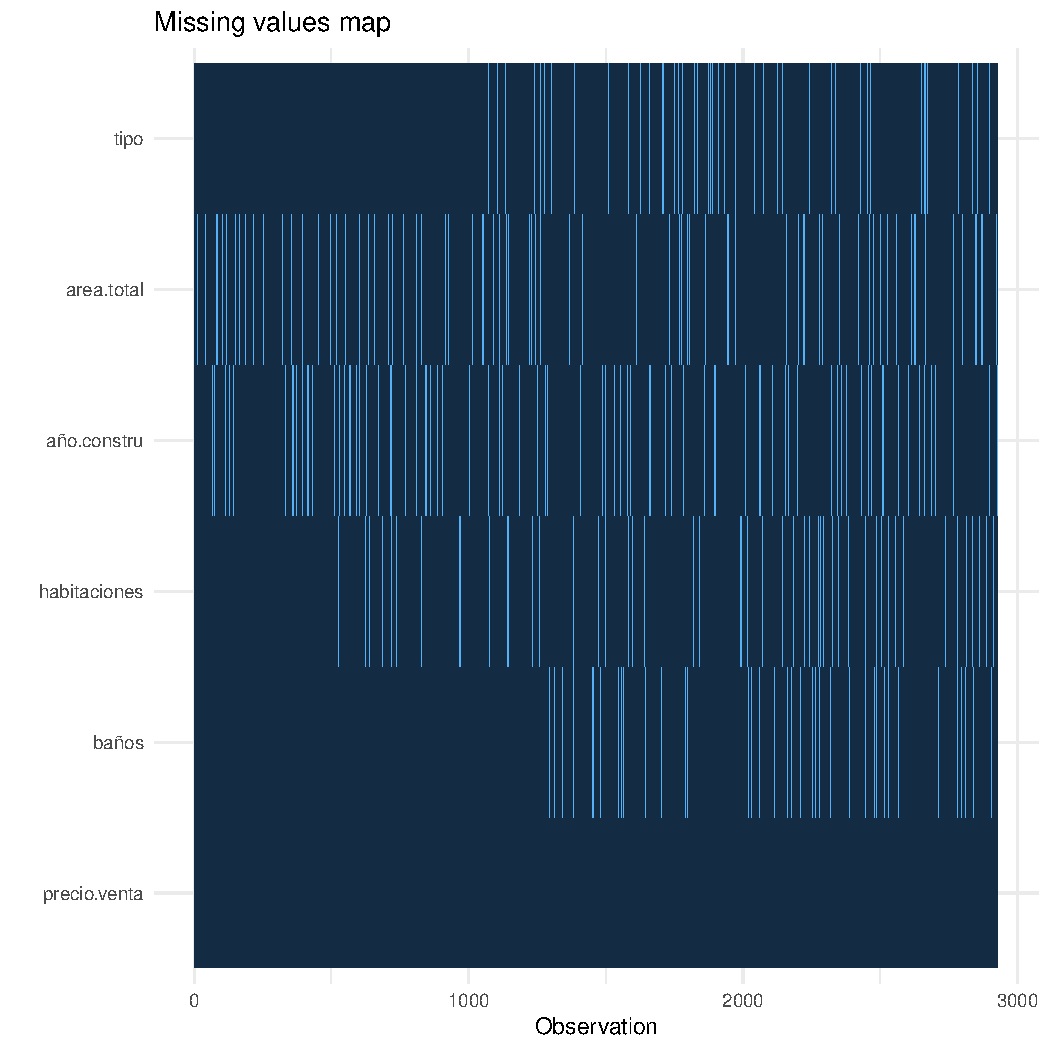
\includegraphics[width=\maxwidth]{figure/unnamed-chunk-3-1} 

\end{knitrout}
    
  \item  Determine el número y porcentaje de valores faltantes, pero esta vez, dentro de cada una de las seis variables. Construya una tabla de resumén de esta información y un gráfico adecuado.
\begin{knitrout}
\definecolor{shadecolor}{rgb}{0.969, 0.969, 0.969}\color{fgcolor}\begin{kframe}
\begin{verbatim}
##              Cantidad de NA'S Porcentaje de NA's
## tipo                      138               4.71
## area.total                267               9.11
## año.constru               288               9.83
## habitaciones              185               6.31
## baños                     106               3.62
## precio.venta                0               0.00
\end{verbatim}
\end{kframe}
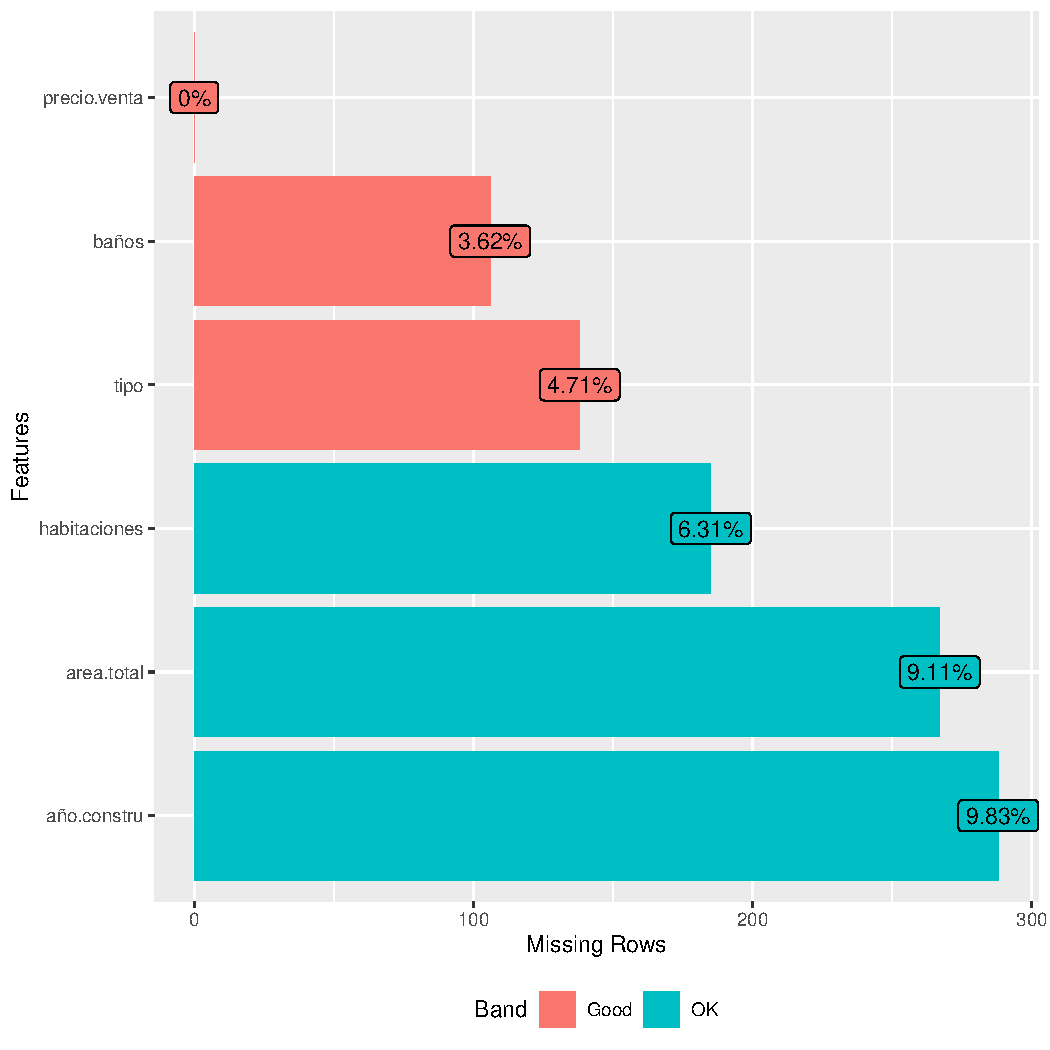
\includegraphics[width=\maxwidth]{figure/unnamed-chunk-4-1} 

\end{knitrout}
   \item Determine el número y el porcentaje de observaciones (fila) con al menos una variable faltante.
\begin{knitrout}
\definecolor{shadecolor}{rgb}{0.969, 0.969, 0.969}\color{fgcolor}\begin{kframe}
\begin{verbatim}
##   Observaciones.NA.s Porcentaje.NA.s
## 1                111        3.788396
\end{verbatim}
\end{kframe}
\end{knitrout}
    \item Determine el número y el porcentaje de observaciones con una, dos, tres, cuatro, cinco o seis valores faltantes (por separado como si fueran categorías). Resuma esta información en un gráfico.
\begin{knitrout}
\definecolor{shadecolor}{rgb}{0.969, 0.969, 0.969}\color{fgcolor}\begin{kframe}
\begin{verbatim}
## # A tibble: 4 x 3
##     NAS total porcentaje
##   <int> <int>      <dbl>
## 1     0  2059    70.3   
## 2     1   760    25.9   
## 3     2   109     3.72  
## 4     3     2     0.0683
\end{verbatim}
\end{kframe}
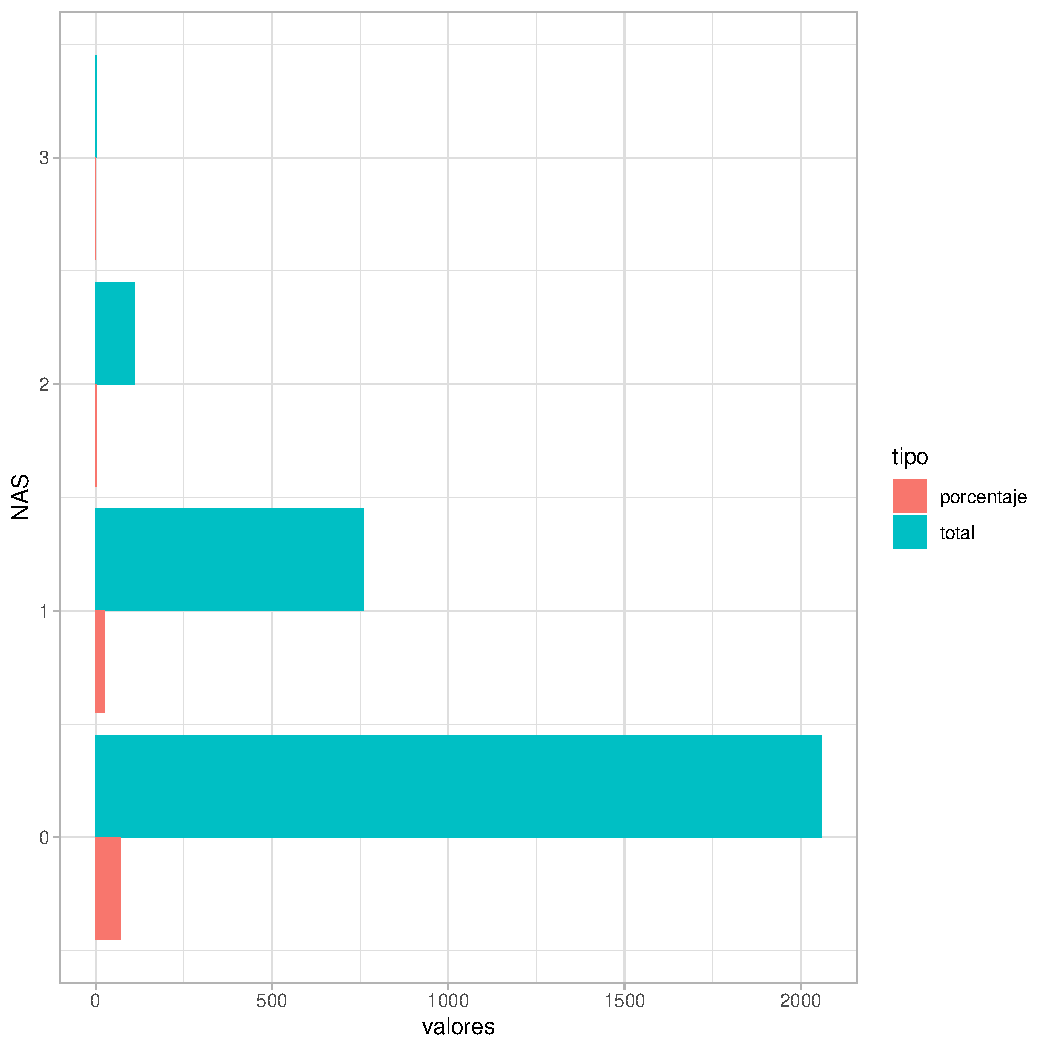
\includegraphics[width=\maxwidth]{figure/unnamed-chunk-6-1} 

\end{knitrout}
 \item  De acuerdo a los resultados obtenidos en las tareas anteriores, tome una decisión: eliminar filas, columnas (ambas) con NA's o aplicar un método de imputación. Justifique su elección.
\\ \\
Al revisar los porentajes de NA's en el conjunto de datos se decide realizar 
 imputación.Se encuentra un gran volumen de NA's, si se eliminará se perderia información en la predicción. \\ \\

  \item  Si la decisión en la trea 6 fue imputar valores, realice esta tarea:
  \begin{enumerate}
      \item [a)] Cree (y presente) una función que permita realizar imputación simple por muestreo aleatorio sin importar el tipo de variable. Aplique esta función al conjunto de datos con NA's.
\begin{knitrout}
\definecolor{shadecolor}{rgb}{0.969, 0.969, 0.969}\color{fgcolor}\begin{kframe}
\begin{alltt}
\hlstd{rand.imput} \hlkwb{<-}\hlkwa{function}\hlstd{(}\hlkwc{x}\hlstd{)\{}
        \hlstd{missing} \hlkwb{<-} \hlstd{(}\hlkwd{is.na}\hlstd{(x))} \hlcom{#vector booleano}
        \hlstd{n.missing} \hlkwb{<-} \hlkwd{sum}\hlstd{(missing)}\hlcom{#Numero de NA’s}
        \hlstd{x.obs} \hlkwb{<-} \hlstd{x[}\hlopt{!}\hlstd{missing]}\hlcom{#Datos no NA}
        \hlstd{imputed} \hlkwb{<-} \hlstd{x}
        \hlstd{imputed[missing]} \hlkwb{<-} \hlkwd{sample}\hlstd{(x.obs,n.missing,}\hlkwc{replace} \hlstd{= T)}
        \hlcom{#Se extrae una muestra aleatoria conocida y se remplazan estos en los NA}
        \hlkwd{return}\hlstd{(imputed)\}}
\hlstd{ventas_casa1}\hlkwb{<-}\hlkwd{data.frame}\hlstd{(}\hlkwc{tipo}\hlstd{=}\hlkwd{rand.imput}\hlstd{(ventas_casas}\hlopt{$}\hlstd{tipo),}
                \hlkwc{area.total}\hlstd{=}\hlkwd{rand.imput}\hlstd{(ventas_casas}\hlopt{$}\hlstd{area.total),}
                \hlkwc{año.constru}\hlstd{=}\hlkwd{rand.imput}\hlstd{(ventas_casas}\hlopt{$}\hlstd{año.constru),}
                \hlkwc{habitaciones}\hlstd{=}\hlkwd{rand.imput}\hlstd{(ventas_casas}\hlopt{$}\hlstd{habitaciones),}
                \hlkwc{baño}\hlstd{=}\hlkwd{rand.imput}\hlstd{(ventas_casas}\hlopt{$}\hlstd{baños))}
\hlkwd{head}\hlstd{(ventas_casa1)}
\end{alltt}
\begin{verbatim}
##          tipo area.total año.constru habitaciones baño
## 1 apartamento      31770        1960            1    1
## 2 apartamento      11622        1961            1    1
## 3 apartamento      14267        2002            1    1
## 4 apartamento      11160        1968            1    1
## 5 apartamento      13830        1997            1    1
## 6 apartamento       9978        1998            1    1
\end{verbatim}
\end{kframe}
\end{knitrout}
 
\begin{knitrout}
\definecolor{shadecolor}{rgb}{0.969, 0.969, 0.969}\color{fgcolor}\begin{kframe}
\begin{alltt}
\hlkwd{tail}\hlstd{(ventas_casa1)}
\end{alltt}
\begin{verbatim}
##      tipo area.total año.constru habitaciones baño
## 2925 casa      20000        1960            1    1
## 2926 casa       7937        1984            1    1
## 2927 casa       8885        1914            1    1
## 2928 casa      10441        1999            1    1
## 2929 casa      10010        1974            1    1
## 2930 casa       9627        1993            2    1
\end{verbatim}
\end{kframe}
\end{knitrout}
     
      \item [b)] Impute los NA's de todas las variables mediante distribuciones no condicionadas (Algoritmo KNN) y,
\begin{knitrout}
\definecolor{shadecolor}{rgb}{0.969, 0.969, 0.969}\color{fgcolor}\begin{kframe}
\begin{alltt}
\hlstd{imputacionKnn}\hlkwb{<-}\hlstd{VIM}\hlopt{::}\hlkwd{kNN}\hlstd{(}\hlkwc{data}\hlstd{=ventas_casas,}
                        \hlkwc{variable} \hlstd{=} \hlkwd{c}\hlstd{(}\hlstr{"tipo"}\hlstd{,}\hlstr{"area.total"}\hlstd{,}\hlstr{"año.constru"}\hlstd{,}\hlstr{"habitaciones"}\hlstd{,}
                                     \hlstr{"baños"}\hlstd{),}
                        \hlkwc{k}\hlstd{=}\hlnum{5}\hlstd{,}\hlkwc{numFun}\hlstd{=mean,}\hlkwc{catFun}\hlstd{=maxCat)}
\hlkwd{head}\hlstd{(imputacionKnn[}\hlnum{1}\hlopt{:}\hlnum{6}\hlstd{])}
\end{alltt}
\begin{verbatim}
##          tipo area.total año.constru habitaciones baños precio.venta
## 1 apartamento      31770        1960            1     1       215000
## 2 apartamento      11622        1961            1     1       105000
## 3 apartamento      14267        1973            1     1       172000
## 4 apartamento      11160        1968            1     1       244000
## 5 apartamento      13830        1997            1     1       189900
## 6 apartamento       9978        1998            1     1       195500
\end{verbatim}
\end{kframe}
\end{knitrout}

\begin{knitrout}
\definecolor{shadecolor}{rgb}{0.969, 0.969, 0.969}\color{fgcolor}\begin{kframe}
\begin{alltt}
\hlkwd{tail}\hlstd{(imputacionKnn[}\hlnum{1}\hlopt{:}\hlnum{6}\hlstd{])}
\end{alltt}
\begin{verbatim}
##      tipo area.total año.constru habitaciones baños precio.venta
## 2925 casa      20000      1960.0          1.0     1       131000
## 2926 casa       7937      1984.0          1.0     1       142500
## 2927 casa       8885      1958.4          1.0     1       131000
## 2928 casa      10441      1937.0          1.0     1       132000
## 2929 casa      10010      1974.0          1.0     1       170000
## 2930 casa       9627      1993.0          1.6     1       188000
\end{verbatim}
\end{kframe}
\end{knitrout}
     
      \item [c)] Impute los NA's de todas las variables mediante imputación múltiple por el algoritmo MICE. 
\begin{knitrout}
\definecolor{shadecolor}{rgb}{0.969, 0.969, 0.969}\color{fgcolor}\begin{kframe}
\begin{alltt}
\hlstd{multimp.mice}\hlkwb{<-}\hlstd{mice}\hlopt{::}\hlkwd{mice}\hlstd{(ventas_casas,}\hlkwc{m} \hlstd{=} \hlnum{5}\hlstd{)}
\end{alltt}
\begin{verbatim}
## 
##  iter imp variable
##   1   1  tipo  area.total  año.constru  habitaciones  baños
##   1   2  tipo  area.total  año.constru  habitaciones  baños
##   1   3  tipo  area.total  año.constru  habitaciones  baños
##   1   4  tipo  area.total  año.constru  habitaciones  baños
##   1   5  tipo  area.total  año.constru  habitaciones  baños
##   2   1  tipo  area.total  año.constru  habitaciones  baños
##   2   2  tipo  area.total  año.constru  habitaciones  baños
##   2   3  tipo  area.total  año.constru  habitaciones  baños
##   2   4  tipo  area.total  año.constru  habitaciones  baños
##   2   5  tipo  area.total  año.constru  habitaciones  baños
##   3   1  tipo  area.total  año.constru  habitaciones  baños
##   3   2  tipo  area.total  año.constru  habitaciones  baños
##   3   3  tipo  area.total  año.constru  habitaciones  baños
##   3   4  tipo  area.total  año.constru  habitaciones  baños
##   3   5  tipo  area.total  año.constru  habitaciones  baños
##   4   1  tipo  area.total  año.constru  habitaciones  baños
##   4   2  tipo  area.total  año.constru  habitaciones  baños
##   4   3  tipo  area.total  año.constru  habitaciones  baños
##   4   4  tipo  area.total  año.constru  habitaciones  baños
##   4   5  tipo  area.total  año.constru  habitaciones  baños
##   5   1  tipo  area.total  año.constru  habitaciones  baños
##   5   2  tipo  area.total  año.constru  habitaciones  baños
##   5   3  tipo  area.total  año.constru  habitaciones  baños
##   5   4  tipo  area.total  año.constru  habitaciones  baños
##   5   5  tipo  area.total  año.constru  habitaciones  baños
\end{verbatim}
\begin{alltt}
\hlstd{imput.mice}\hlkwb{<-}\hlkwd{complete}\hlstd{(multimp.mice)}
\hlkwd{head}\hlstd{(imput.mice)}
\end{alltt}
\begin{verbatim}
##          tipo area.total año.constru habitaciones baños precio.venta
## 1 apartamento      31770        1960            1     1       215000
## 2 apartamento      11622        1961            1     1       105000
## 3 apartamento      14267        1978            1     1       172000
## 4 apartamento      11160        1968            1     1       244000
## 5 apartamento      13830        1997            1     1       189900
## 6 apartamento       9978        1998            1     1       195500
\end{verbatim}
\end{kframe}
\end{knitrout}

\begin{knitrout}
\definecolor{shadecolor}{rgb}{0.969, 0.969, 0.969}\color{fgcolor}\begin{kframe}
\begin{alltt}
\hlkwd{tail}\hlstd{(imput.mice)}
\end{alltt}
\begin{verbatim}
##      tipo area.total año.constru habitaciones baños precio.venta
## 2925 casa      20000        1960            1     1       131000
## 2926 casa       7937        1984            1     1       142500
## 2927 casa       8885        1965            1     1       131000
## 2928 casa      10441        1970            1     1       132000
## 2929 casa      10010        1974            1     1       170000
## 2930 casa       9627        1993            1     1       188000
\end{verbatim}
\end{kframe}
\end{knitrout}
      
      \\ \\
\textbf{¿Cuál de las tres imputaciones es la más eficiente y adecuada para usted? Argumente y justifique su elección mostrando evidencia numérica o gráfica }
\\ \\
Se utiliza el test kolmogorov smirnov para las variables numericas y un test chi-cuadrado para las variables categoricas y así determinar si la distribución de los datos ha cambiado al realizar las imputaciones. \\ \\
\textbf{Sistema de hipotesis de la prueba Kolmogorov-smirnov} \\ \\
\(H_o: X\) proviene de un modelo probabilistico particular con función de distribución $F(x)$. \\ 
\(H_a:X\) proviene de cualquier otro modelo probabilistico con función de distribución $G(x)\neq F(X).$ \\ 
Matematicamente,este sistema de hipotesis se traduce a:
\[H_o: F(X) = F^{*}(X) \]
\[H_a: F(X) \neq F^{*}(X) \]
\textbf{Sistema de hipotesis de la prueba chi-cuadrado} \\ \\
\[H_o: O_i = E_i \]
\[H_a: O_i \neq E_i) \]
\textbf{Pruebas de bondad de ajuste para los valores imputados por el muestreo aleatorio simple} 
\begin{knitrout}
\definecolor{shadecolor}{rgb}{0.969, 0.969, 0.969}\color{fgcolor}\begin{kframe}
\begin{alltt}
\hlkwd{chisq.test}\hlstd{(}\hlkwc{x}\hlstd{=ventas_casas}\hlopt{$}\hlstd{tipo,}\hlkwc{y}\hlstd{=ventas_casa1}\hlopt{$}\hlstd{tipo)}
\end{alltt}
\begin{verbatim}
## 
## 	Pearson's Chi-squared test
## 
## data:  ventas_casas$tipo and ventas_casa1$tipo
## X-squared = 5584, df = 4, p-value < 2.2e-16
\end{verbatim}
\begin{alltt}
\hlkwd{ks.test}\hlstd{(}\hlkwc{x}\hlstd{=ventas_casas}\hlopt{$}\hlstd{area.total,}\hlkwc{y}\hlstd{=ventas_casa1}\hlopt{$}\hlstd{area.total)}
\end{alltt}
\begin{verbatim}
## 
## 	Two-sample Kolmogorov-Smirnov test
## 
## data:  ventas_casas$area.total and ventas_casa1$area.total
## D = 0.0050108, p-value = 1
## alternative hypothesis: two-sided
\end{verbatim}
\begin{alltt}
\hlkwd{ks.test}\hlstd{(}\hlkwc{x}\hlstd{=ventas_casas}\hlopt{$}\hlstd{año.constru,}\hlkwc{y}\hlstd{=ventas_casa1}\hlopt{$}\hlstd{año.constru)}
\end{alltt}
\begin{verbatim}
## 
## 	Two-sample Kolmogorov-Smirnov test
## 
## data:  ventas_casas$año.constru and ventas_casa1$año.constru
## D = 0.0049582, p-value = 1
## alternative hypothesis: two-sided
\end{verbatim}
\begin{alltt}
\hlkwd{ks.test}\hlstd{(}\hlkwc{x}\hlstd{=ventas_casas}\hlopt{$}\hlstd{habitaciones,}\hlkwc{y}\hlstd{=ventas_casa1}\hlopt{$}\hlstd{habitaciones)}
\end{alltt}
\begin{verbatim}
## 
## 	Two-sample Kolmogorov-Smirnov test
## 
## data:  ventas_casas$habitaciones and ventas_casa1$habitaciones
## D = 0.0034981, p-value = 1
## alternative hypothesis: two-sided
\end{verbatim}
\begin{alltt}
\hlcom{#ks.test(x=ventas_casas$baños,y=ventas_casa1$baños)}
\end{alltt}
\end{kframe}
\end{knitrout}
  No se rechaza la hipotesis nuela en las pruebas kolmogorov.\\ \\
   \textbf{Pruebas de bondad de ajuste para los valores imputados por el metodo KNN} 
\begin{knitrout}
\definecolor{shadecolor}{rgb}{0.969, 0.969, 0.969}\color{fgcolor}\begin{kframe}
\begin{alltt}
\hlkwd{chisq.test}\hlstd{(}\hlkwc{x}\hlstd{=ventas_casas}\hlopt{$}\hlstd{tipo,}\hlkwc{y}\hlstd{=imputacionKnn}\hlopt{$}\hlstd{tipo)}
\end{alltt}
\begin{verbatim}
## 
## 	Pearson's Chi-squared test
## 
## data:  ventas_casas$tipo and imputacionKnn$tipo
## X-squared = 5584, df = 4, p-value < 2.2e-16
\end{verbatim}
\begin{alltt}
\hlkwd{ks.test}\hlstd{(}\hlkwc{x}\hlstd{=ventas_casas}\hlopt{$}\hlstd{area.total,}\hlkwc{y}\hlstd{=imputacionKnn}\hlopt{$}\hlstd{area.total)}
\end{alltt}
\begin{verbatim}
## 
## 	Two-sample Kolmogorov-Smirnov test
## 
## data:  ventas_casas$area.total and imputacionKnn$area.total
## D = 0.009259, p-value = 0.9998
## alternative hypothesis: two-sided
\end{verbatim}
\begin{alltt}
\hlkwd{ks.test}\hlstd{(}\hlkwc{x}\hlstd{=ventas_casas}\hlopt{$}\hlstd{año.constru,}\hlkwc{y}\hlstd{=imputacionKnn}\hlopt{$}\hlstd{año.constru)}
\end{alltt}
\begin{verbatim}
## 
## 	Two-sample Kolmogorov-Smirnov test
## 
## data:  ventas_casas$año.constru and imputacionKnn$año.constru
## D = 0.013381, p-value = 0.9647
## alternative hypothesis: two-sided
\end{verbatim}
\begin{alltt}
\hlkwd{ks.test}\hlstd{(}\hlkwc{x}\hlstd{=ventas_casas}\hlopt{$}\hlstd{habitaciones,}\hlkwc{y}\hlstd{=imputacionKnn}\hlopt{$}\hlstd{habitaciones)}
\end{alltt}
\begin{verbatim}
## 
## 	Two-sample Kolmogorov-Smirnov test
## 
## data:  ventas_casas$habitaciones and imputacionKnn$habitaciones
## D = 0.023293, p-value = 0.4254
## alternative hypothesis: two-sided
\end{verbatim}
\begin{alltt}
\hlkwd{ks.test}\hlstd{(}\hlkwc{x}\hlstd{=ventas_casas}\hlopt{$}\hlstd{baños,}\hlkwc{y}\hlstd{=imputacionKnn}\hlopt{$}\hlstd{baños)}
\end{alltt}
\begin{verbatim}
## 
## 	Two-sample Kolmogorov-Smirnov test
## 
## data:  ventas_casas$baños and imputacionKnn$baños
## D = 0.017249, p-value = 0.7857
## alternative hypothesis: two-sided
\end{verbatim}
\end{kframe}
\end{knitrout}

No se rechaza la hipotesis nula en las pruebas kolmogorov y el valor p es muy cercano a 1,es decir que la distribución de los datos teorica es igual a la impirica que se obtuvo al imputar por el método KNN. \\ \\
   \textbf{Pruebas de bondad de ajuste para los valores imputados por el metodo MICE} 
\begin{knitrout}
\definecolor{shadecolor}{rgb}{0.969, 0.969, 0.969}\color{fgcolor}\begin{kframe}
\begin{alltt}
\hlkwd{chisq.test}\hlstd{(}\hlkwc{x}\hlstd{=ventas_casas}\hlopt{$}\hlstd{tipo,}\hlkwc{y}\hlstd{=imput.mice}\hlopt{$}\hlstd{tipo)}
\end{alltt}
\begin{verbatim}
## 
## 	Pearson's Chi-squared test
## 
## data:  ventas_casas$tipo and imput.mice$tipo
## X-squared = 5584, df = 4, p-value < 2.2e-16
\end{verbatim}
\begin{alltt}
\hlkwd{ks.test}\hlstd{(}\hlkwc{x}\hlstd{=ventas_casas}\hlopt{$}\hlstd{area.total,}\hlkwc{y}\hlstd{=imput.mice}\hlopt{$}\hlstd{area.total)}
\end{alltt}
\begin{verbatim}
## 
## 	Two-sample Kolmogorov-Smirnov test
## 
## data:  ventas_casas$area.total and imput.mice$area.total
## D = 0.0044958, p-value = 1
## alternative hypothesis: two-sided
\end{verbatim}
\begin{alltt}
\hlkwd{ks.test}\hlstd{(}\hlkwc{x}\hlstd{=ventas_casas}\hlopt{$}\hlstd{año.constru,}\hlkwc{y}\hlstd{=imput.mice}\hlopt{$}\hlstd{año.constru)}
\end{alltt}
\begin{verbatim}
## 
## 	Two-sample Kolmogorov-Smirnov test
## 
## data:  ventas_casas$año.constru and imput.mice$año.constru
## D = 0.0043392, p-value = 1
## alternative hypothesis: two-sided
\end{verbatim}
\begin{alltt}
\hlkwd{ks.test}\hlstd{(}\hlkwc{x}\hlstd{=ventas_casas}\hlopt{$}\hlstd{habitaciones,}\hlkwc{y}\hlstd{=imput.mice}\hlopt{$}\hlstd{habitaciones)}
\end{alltt}
\begin{verbatim}
## 
## 	Two-sample Kolmogorov-Smirnov test
## 
## data:  ventas_casas$habitaciones and imput.mice$habitaciones
## D = 0.0024742, p-value = 1
## alternative hypothesis: two-sided
\end{verbatim}
\begin{alltt}
\hlkwd{ks.test}\hlstd{(}\hlkwc{x}\hlstd{=ventas_casas}\hlopt{$}\hlstd{baños,}\hlkwc{y}\hlstd{=imput.mice}\hlopt{$}\hlstd{baños)}
\end{alltt}
\begin{verbatim}
## 
## 	Two-sample Kolmogorov-Smirnov test
## 
## data:  ventas_casas$baños and imput.mice$baños
## D = 0.0042793, p-value = 1
## alternative hypothesis: two-sided
\end{verbatim}
\end{kframe}
\end{knitrout}
   No se rechaza la hipotesis nula en las pruebas kolmogorov y el valor p es 1,es decir que la distribución de los datos teorica es igual a la impirica que se obtuvo al imputar por el método MICE. \\ \\
El mejor metodo de imputación fue imputacion multivariada por ecuaciones encadenadas(MICE),ya que al realizar pruebas de bondad de ajuste entre la distribución teorica de los datos para cada variable y la distribución empirica(la imputada por el metodo MICE) se evidencia que las distribuciónes de las variables no difieren y su valor p es 1.
      
  \end{enumerate}
   \item  Con los datos ya imputados (por el método que usted escogió como el mejor),ajuste un modelo lineal de regresión múltiple tomando como una variable de respuesta (Precio.venta) y como variable explicativa las demás variables.Reporte el modelo ajustado (con coeficiente de regresión estimados).
\begin{knitrout}
\definecolor{shadecolor}{rgb}{0.969, 0.969, 0.969}\color{fgcolor}\begin{kframe}
\begin{alltt}
\hlstd{train}\hlkwb{<-}\hlstd{imput.mice}\hlopt\hlkwd{mutate}\hlstd{(}\hlkwc{precio.venta}\hlstd{=}\hlkwd{factor}\hlstd{(precio.venta))}

\hlstd{modelo}\hlkwb{<-}\hlkwd{lm}\hlstd{(}\hlkwc{formula} \hlstd{= precio.venta}\hlopt{~}\hlkwd{as.factor}\hlstd{(tipo)}\hlopt{+}\hlstd{area.total}\hlopt{+}\hlstd{año.constru}\hlopt{+}
                \hlstd{habitaciones}\hlopt{+}\hlstd{baños,}\hlkwc{data}\hlstd{=train)}
\hlkwd{round}\hlstd{(}\hlkwd{coef}\hlstd{(modelo),}\hlnum{2}\hlstd{)}
\end{alltt}
\begin{verbatim}
##           (Intercept)   as.factor(tipo)casa as.factor(tipo)Duplex 
##              -4367.00                 -3.94               -136.59 
##            area.total           año.constru          habitaciones 
##                  0.01                  2.41                 -6.09 
##                 baños 
##                 -9.15
\end{verbatim}
\end{kframe}
\end{knitrout}
   
    \item Prediga el precio de venta de los siguientes inmuebles con base en el modelo ajustado en el item anterior,y sus correspondientes perfiles, y complete esta tabla:
\begin{knitrout}
\definecolor{shadecolor}{rgb}{0.969, 0.969, 0.969}\color{fgcolor}\begin{kframe}
\begin{alltt}
\hlstd{new}\hlkwb{<-}\hlkwd{data.frame}\hlstd{(}\hlkwc{tipo}\hlstd{=}\hlkwd{as.factor}\hlstd{(}\hlkwd{c}\hlstd{(}\hlstr{"apartamento"}\hlstd{,}\hlstr{"apartamento"}\hlstd{,}\hlstr{"casa"}\hlstd{,}\hlstr{"Duplex"}\hlstd{)),}
\hlkwc{area.total}\hlstd{=}\hlkwd{c}\hlstd{(}\hlnum{12567}\hlstd{,}\hlnum{45250}\hlstd{,}\hlnum{100225}\hlstd{,}\hlnum{8066}\hlstd{),}\hlkwc{año.constru}\hlstd{=}\hlkwd{c}\hlstd{(}\hlnum{1965}\hlstd{,}\hlnum{2010}\hlstd{,}\hlnum{1905}\hlstd{,}\hlnum{1942}\hlstd{),}
\hlkwc{habitaciones}\hlstd{=}\hlkwd{c}\hlstd{(}\hlnum{2}\hlstd{,}\hlnum{2}\hlstd{,}\hlnum{1}\hlstd{,}\hlnum{4}\hlstd{),}\hlkwc{baños}\hlstd{=}\hlkwd{c}\hlstd{(}\hlnum{1}\hlstd{,}\hlnum{2}\hlstd{,}\hlnum{1}\hlstd{,}\hlnum{2}\hlstd{))}

\hlstd{prediccion}\hlkwb{<-}\hlkwd{predict}\hlstd{(}\hlkwc{object} \hlstd{= modelo,}\hlkwc{newdata} \hlstd{= new)}
\hlkwd{cbind}\hlstd{(new,prediccion)}
\end{alltt}
\begin{verbatim}
##          tipo area.total año.constru habitaciones baños prediccion
## 1 apartamento      12567        1965            2     1   455.1718
## 2 apartamento      45250        2010            2     2   831.3126
## 3        casa     100225        1905            1     1  1055.1048
## 4      Duplex       8066        1942            4     2   203.6749
\end{verbatim}
\end{kframe}
\end{knitrout}
    
\end{enumerate}

\bibliographystyle{apacite}
\bibliography{mineria.bib}

\\
Ramos, D.  (2020).\textit{Detección y tratamiento de datosfaltantes: missing data}

\end{document}
